\documentclass[../../main.tex]{subfiles}
\begin{document}
{\bf[解]}

与えられた曲線の関数を
\begin{align}
  f(x) = \dfrac{3}{2}x^2-\dfrac{1}{3} \label{eq:1}
\end{align}
とおく．一階微分は
\begin{align}
  f'(x) = 3x
\end{align}
だから，$C(t,f(t))$における法線は
\begin{align}
  & (x-t)+3t\left(y-\dfrac{3}{2}t^2+\dfrac{1}{3}\right)=0 \nonumber\\
  \therefore
  & 9t^3-6yt-2x=0 \label{eq:2}
\end{align}
である．

\begin{figure}[htb]
  \centering
  \begin{tikzpicture}[scale=2.2, >=stealth, every node/.style={font=\small}]

    % --- 1. 定数・接点パラメータの定義 ---
    % f(x) = 3/2 * x^2 - 1/3
    % f'(x) = 3x
    % 接点 C のパラメータ: t = 0.70 とする
    \def\tVal{0.70}
    \pgfmathsetmacro{\yC}{1.5*\tVal*\tVal - 1.0/3.0} % f(t) = 1.5*(0.49) - 0.3333 ≈ 0.4017
    \pgfmathsetmacro{\mTan}{3.0*\tVal}               % 接線の傾き f'(t) = 2.10
    \pgfmathsetmacro{\mNorm}{-1.0/\mTan}             % 法線の傾き -1/(3t) ≈ -0.4762

    % 座標定義
    \coordinate (O) at (0, 0);
    \coordinate (C) at (\tVal, \yC);                 % 接点 C(t, f(t))

    % --- 2. 座標軸 ---
    \draw[->, thick] (-1.4, 0) -- (1.6, 0) node[right] {$x$};
    \draw[->, thick] (0, -0.6) -- (0, 1.6) node[above] {$y$};
    \node[below left=2pt] at (O) {$O$};

    % --- 3. 放物線 y = f(x) = 3/2 x^2 - 1/3 ---
    \draw[very thick, blue!85!black, domain=-1.1:1.1, samples=80]
    plot (\x, {1.5*\x*\x - 1.0/3.0});
    \node[blue!85!black, font=\footnotesize, right] at (1.05, 1.35) {$y = \dfrac{3}{2}x^2 - \dfrac{1}{3}$};

    % --- 4. 接線 (参考線) ---
    % 接線方程式: y - yC = mTan * (x - t)
    \draw[thick, dashed, gray!60, domain=0.35:1.05]
    plot (\x, {\yC + \mTan*(\x - \tVal)});
    \node[gray!70!black, font=\scriptsize, above left] at (1.05, {\yC + \mTan*(1.05 - \tVal)}) {接線};

    % --- 5. 法線 (主役線) ---
    % 法線方程式: (x - t) + 3t(y - f(t)) = 0 <=> y - yC = mNorm * (x - t)
    \draw[very thick, red!85!black, domain=-0.9:1.4]
    plot (\x, {\yC + \mNorm*(\x - \tVal)});
    \node[red!85!black, font=\footnotesize, below left] at (-0.6, {\yC + \mNorm*(-0.6 - \tVal)}) {法線};

    % --- 6. 接点における直角マーク ---
    % 接線方向ベクトル: (1, mTan) を正規化
    % 法線方向ベクトル: (1, mNorm) を正規化
    \pgfmathsetmacro{\lenTan}{sqrt(1.0 + \mTan*\mTan)}
    \pgfmathsetmacro{\lenNorm}{sqrt(1.0 + \mNorm*\mNorm)}
    \pgfmathsetmacro{\uTx}{1.0 / \lenTan * 0.08}
    \pgfmathsetmacro{\uTy}{\mTan / \lenTan * 0.08}
    \pgfmathsetmacro{\uNx}{-1.0 / \lenNorm * 0.08}
    \pgfmathsetmacro{\uNy}{-\mNorm / \lenNorm * 0.08}

    \draw[gray!80!black]
    ($ (C) + (\uTx, \uTy) $) --
    ($ (C) + (\uTx + \uNx, \uTy + \uNy) $) --
    ($ (C) + (\uNx, \uNy) $);

    % --- 7. 主要点・法線上の点 P(X, Y) の配置 ---
    % 接点 C(t, f(t))
    \fill[blue!85!black] (C) circle (0.9pt);
    \node[right=2pt, font=\footnotesize, blue!85!black] at (C) {$C(t, f(t))$};

    % 接点の座標射影
    \draw[dotted, gray!70] (\tVal, 0) -- (C) -- (0, \yC);
    \fill (\tVal, 0) circle (0.6pt);
    \node[below=2pt, font=\scriptsize] at (\tVal, 0) {$t$};
    \fill (0, \yC) circle (0.6pt);
    \node[left=2pt, font=\scriptsize] at (0, \yC) {$f(t)$};

    % y 切片 (0, -1/3)
    \fill (0, -0.3333) circle (0.6pt);
    \node[left=2pt, font=\scriptsize] at (0, -0.3333) {$-\dfrac{1}{3}$};

    % 法線上の任意の点 P(X, Y)
    \def\xP{-0.3}
    \pgfmathsetmacro{\yP}{\yC + \mNorm*(\xP - \tVal)}
    \coordinate (P) at (\xP, \yP);
    \fill[red!80!black] (P) circle (1.0pt);
    \node[above=2pt, font=\footnotesize, red!80!black] at (P) {$P(X, Y)$};

    % 点 P からの補助線
    \draw[dashed, red!60] (\xP, 0) -- (P) -- (0, \yP);
    \node[below=2pt, font=\scriptsize, red!80!black] at (\xP, 0) {$X$};
    \node[left=2pt, font=\scriptsize, red!80!black] at (0, \yP) {$Y$};

  \end{tikzpicture}
  \caption{放物線 $y = f(x)$ 上の点 $C(t, f(t))$ における法線と通過する点 $P(X, Y)$}
  \label{fig:parabola_normal_overview}
\end{figure}

\paragraph{(1)}

点$P(X,Y)$とおく．放物線では接点が異なれば法線が異なるから，点Pに対して\cref{eq:2}を満たす$t$がただ一つ存在すればよい．そこで\cref{eq:2}に$(x,y)=(X,Y)$を代入して
\begin{align}
  g(t) = 9t^3-6Yt-2X=0 \label{eq:3}
\end{align}
について考える．一階微分は
\begin{align}
  g'(t)=27t^2-6Y \label{eq:4}
\end{align}
だから，$Y$の値に応じて$g(t)$の挙動は以下のように変化する．

\subparagraph{(i)$Y\le0$の時}

この時は\cref{eq:4}より$g'(t)\ge0$だから$g(t)$は単調増加である．
$g(t)$は$3$次関数だから$g(t)=0$は唯一つ解を持つ．

\subparagraph{(ii)$Y>0$の時}

この時は\cref{eq:4}は必ず二つの零点をもち，$g(t)$の増減表は以下のようになる．
ただし$\alpha=\dfrac{\sqrt{2y}}{3}$とおいた．

\begin{table}[htb]
  \centering
  \caption{$g(t)$ の増減表}
  \label{tab:g_increase_decrease}
  \renewcommand{\arraystretch}{1.3}
  \begin{tabular}{c|ccccc}
    $t$ & $\cdots$ & $-\alpha$ & $\cdots$ & $\alpha$ & $\cdots$ \\
    \hline
    $g'(t)$ & $+$ & $0$ & $-$ & $0$ & $+$ \\
    \hline
    $g(t)$ & $\nearrow$ & 極大 & $\searrow$ & 極小 & $\nearrow$
  \end{tabular}
\end{table}

従って，$g(t)$のグラフの概形は下図のようになる．

\begin{figure}[htb]
  \centering
  \begin{tikzpicture}[scale=1.5, >=stealth, every node/.style={font=\small}]

    % --- 1. 定数・極値パラメータの定義 ---
    % g(t) = 9t^3 - 6Yt - 2X  (Y > 0)
    % g'(t) = 27t^2 - 6Y = 0 <=> t = ±sqrt(2Y)/3 = ±\alpha
    % 例として \alpha = 1.0, 2X = 0.5 (Y 切片が -2X) と設定
    \def\alphaVal{1.0}
    \def\twoX{0.45}

    % 極大値: g(-\alpha) = 4Y\alpha - 2X
    % 極小値: g(\alpha)  = -4Y\alpha - 2X
    \pgfmathsetmacro{\yMax}{2.0 - \twoX}   % 極大値
    \pgfmathsetmacro{\yMin}{-2.0 - \twoX}  % 極小値
    \pgfmathsetmacro{\yIntercept}{-\twoX}  % t = 0 の切片 -2X

    % --- 2. 座標軸 (横軸: t, 縦軸: y) ---
    \draw[->, thick] (-1.9, 0) -- (2.2, 0) node[right] {$t$};
    \draw[->, thick] (0, -3.2) -- (0, 2.5) node[above] {$y$};
    \node[above left=2pt] at (0, 0) {$O$};

    % --- 3. グラフ y = g(t) の描画 ---
    % 標準的な3次曲線: y = 2*(t/\alpha)^3 - 3*(t/\alpha) - 2X の形状にスケーリング
    \draw[line width=1.3pt, blue!85!black, domain=-1.8:1.9, samples=100]
    plot (\x, { (\x/\alphaVal)*(\x/\alphaVal)*(\x/\alphaVal) - 3*(\x/\alphaVal) - \twoX });
    \node[blue!85!black, font=\normalsize\bfseries, right] at (1.4, 1.8) {$y = g(t)$};

    % --- 4. 極大点・極小点の補助線とプロット ---
    % (i) 極大点: t = -\alpha
    \draw[dashed, gray!70] (-\alphaVal, 0) -- (-\alphaVal, \yMax) -- (0, \yMax);
    \fill[red!80!black] (-\alphaVal, \yMax) circle (1.2pt);
    \node[below=2pt, font=\footnotesize, red!80!black] at (-\alphaVal, 0) {$-\alpha$};
    \node[right=2pt, font=\scriptsize, red!80!black] at (0, \yMax) {$g(-\alpha)$};

    % (ii) 極小点: t = \alpha
    \draw[dashed, gray!70] (\alphaVal, 0) -- (\alphaVal, \yMin) -- (0, \yMin);
    \fill[red!80!black] (\alphaVal, \yMin) circle (1.2pt);
    \node[above=2pt, font=\footnotesize, red!80!black] at (\alphaVal, 0) {$\alpha$};
    \node[left=2pt, font=\scriptsize, red!80!black] at (0, \yMin) {$g(\alpha)$};

    % --- 5. 切片のプロットとラベル ---
    % y 切片 (0, -2X)
    \fill (0, \yIntercept) circle (1.0pt);
    \node[above right=1pt, font=\footnotesize] at (0, \yIntercept) {$-2X$};

    % --- 6. 定義・極値の注記 ---
    \node[draw=gray!60, fill=white, rounded corners=2pt, inner sep=3pt, font=\scriptsize, align=left]
    at (-1.25, -2.4) {$\alpha = \dfrac{\sqrt{2Y}}{3}$};

  \end{tikzpicture}
  \caption{$Y > 0$ における $y = g(t) = 9t^3 - 6Yt - 2X$ の概形}
  \label{fig:graph_gt_cubic}
\end{figure}

図より$g(t)=0$がただ一つの解を持つ条件は
\begin{align}
  g(-\alpha)g(\alpha)>0 \label{eq:5}
\end{align}
である．ここで\cref{eq:3}から
\begin{align}
  g(\pm\alpha)&=\pm 9\alpha^3\mp 6y\alpha -2x \\
  &=\mp \dfrac{4\sqrt{2}}{3}y^{3/2}-2x
\end{align}
であるから，\cref{eq:5}に代入して
\begin{align}
  \left(\dfrac{2\sqrt{2}}{3}y^{3/2}-x\right)\left(-\dfrac{2\sqrt{2}}{3}y^{3/2}-x\right)>0\label{eq:6}
\end{align}
である．以上から求める条件は

以上から，求める領域は，
\begin{align}
  y\le0 \lor(y>0 \land \text{\cref{eq:6}})
\end{align}
であって，図示すると下図斜線部(境界含む)である．$\cdots$((1)の答)

\begin{figure}[htb]
  \centering
  \begin{tikzpicture}[scale=1.6, >=stealth, every node/.style={font=\small}]

    % --- 1. クリッピング枠の設定 ---
    \clip (-2.6, -1.6) rectangle (2.6, 2.5);

    % --- 2. 境界曲線・領域の定義 ---
    % 条件式:
    % (i)  Y <= 0 (下半平面全体)
    % (ii) Y > 0 において:
    %      ( 2*sqrt(2)/3 * Y^(3/2) - X ) * ( -2*sqrt(2)/3 * Y^(3/2) - X ) >= 0
    %      <=> X^2 - 8/9 * Y^3 >= 0  <=>  Y <= (9/8 * X^2)^(1/3) = (3/2)^(2/3) * |X|^(2/3)
    %      境界曲線: 半立方放物線 (Cusp): 27X^2 = 8Y^3 <=> Y = (9/8)^(1/3) * |X|^(2/3)

    % (1) Y <= 0 の領域（下半平面）のハッチング
    \fill[pattern=north east lines, pattern color=blue!50]
    (-2.6, -1.6) rectangle (2.6, 0);

    % (2) Y > 0 かつ |X| >= 2*sqrt(2)/3 * Y^(3/2) の領域のハッチング
    % 左側領域 (X <= 0):
    \fill[pattern=north east lines, pattern color=blue!50]
    (-2.6, 0) -- plot[domain=0:2.1, variable=\y, samples=80] ({-2*sqrt(2)/3 * (\y)^(1.5)}, \y)
    -- (-2.6, 2.1) -- cycle;

    % 右側領域 (X >= 0):
    \fill[pattern=north east lines, pattern color=blue!50]
    (2.6, 0) -- plot[domain=0:2.1, variable=\y, samples=80] ({2*sqrt(2)/3 * (\y)^(1.5)}, \y)
    -- (2.6, 2.1) -- cycle;

    % --- 3. 境界曲線の描画 (半立方放物線: 尖点をもつ曲線) ---
    % 右側分枝: X = 2*sqrt(2)/3 * Y^(3/2)
    \draw[very thick, teal!85!black, domain=0:2.3, variable=\y, samples=100]
    plot ({2*sqrt(2)/3 * (\y)^(1.5)}, \y);

    % 左側分枝: X = -2*sqrt(2)/3 * Y^(3/2)
    \draw[very thick, teal!85!black, domain=0:2.3, variable=\y, samples=100]
    plot ({-2*sqrt(2)/3 * (\y)^(1.5)}, \y);

    % X軸上の境界線 (Y <= 0 との境界)
    \draw[very thick, teal!85!black] (-2.6, 0) -- (2.6, 0);

    % --- 4. 座標軸 ---
    \draw[->, thick] (-2.6, 0) -- (2.7, 0) node[right] {$X$};
    \draw[->, thick] (0, -1.6) -- (0, 2.5) node[above] {$Y$};
    \node[above left=2pt] at (0, 0) {$O$};

    % --- 5. 境界曲線のラベル ---
    \node[teal!85!black, font=\footnotesize, right] at (1.2, 1.8) {$X^2 = \dfrac{8}{9}Y^3$};

    % 尖点 (原点) の注記
    \fill[red!80!black] (0, 0) circle (1.2pt);

  \end{tikzpicture}
  \caption{法線がただ1本存在する点 $P(X, Y)$ の動く領域（斜線部，境界を含む）}
  \label{fig:normal_unique_region}
\end{figure}

\paragraph{(2)}
この領域の対称性から$x\ge0$の部分の面積$S_1$とすると，求める面積$S$との関係は
\begin{align}
  S=2S_1 \label{eq:7}
\end{align}
である．$y=f(x)$と$x=\dfrac{2\sqrt{2}}{3}y^{3/2}$の$y>0$での交点は，
\begin{align}
  &y=\dfrac{3}{2}\left(\dfrac{2\sqrt{2}}{3}y^{3/2}\right)^2-\dfrac{1}{3} \\
  &4y^3-3y-1=0 \\
  &(y-1)(4y^2+4y+1)=0 \\
  &y=1&(\because y>0)
\end{align}
である．このとき$x=\dfrac{2\sqrt{2}}{3}(\equiv \beta)$である．よってグラフの概形は下図の斜線部となる．

\begin{figure}[htb]
  \centering
  \begin{tikzpicture}[scale=2.6, >=stealth, every node/.style={font=\small}]

    % --- 1. 定数・交点パラメータの定義 ---
    % 交点: y = 1, x = 2*sqrt(2)/3 ≈ 0.9428 (beta)
    % f(x) = 3/2 * x^2 - 1/3
    % x 切片 (f(x) = 0): x = sqrt(2)/3 ≈ 0.4714
    % y 切片: (0, -1/3)
    \def\betaVal{0.9428}
    \def\xZero{0.4714}

    % --- 2. 面積 S_1 (x >= 0) のハッチング領域 ---
    % 積分区間・囲まれる領域:
    % 上側 / 左側: 放物線 y = 3/2*x^2 - 1/3 (x 切片 sqrt(2)/3 から 交点 beta まで)
    % 下側 / 右側: 半立方放物線 x = 2*sqrt(2)/3 * y^(3/2) <=> y = (9/8 * x^2)^(1/3) (0 <= y <= 1)
    \fill[pattern=north east lines, pattern color=blue!60]
    (0,-1/3)
    -- plot[domain=0:\betaVal, samples=60] (\x, {1.5*\x*\x - 1.0/3.0})
    -- plot[domain=1.0:0, variable=\y, samples=60] ({2.0*sqrt(2)/3.0 * (\y)^(1.5)}, \y)
    -- cycle;

    % --- 3. 座標軸 ---
    \draw[->, thick] (-1.5, 0) -- (1.5, 0) node[right] {$x$};
    \draw[->, thick] (0, -0.6) -- (0, 1.45) node[above] {$y$};
    \node[below left=2pt] at (0, 0) {$O$};

    % --- 4. 曲線群の描画 ---
    % (i) 放物線 y = f(x) = 3/2*x^2 - 1/3
    \draw[very thick, blue!85!black, domain=-1.05:1.05, samples=80]
    plot (\x, {1.5*\x*\x - 1.0/3.0});
    \node[blue!85!black, font=\footnotesize, right] at (1.0, 1.25) {$y = f(x)$};

    % (ii) 半立方放物線の右分枝: x = 2*sqrt(2)/3 * y^(3/2)
    \draw[very thick, teal!85!black, domain=0:1.25, variable=\y, samples=80]
    plot ({2.0*sqrt(2)/3.0 * (\y)^(1.5)}, \y);
    \node[teal!85!black, font=\footnotesize, right] at (1.1, 0.9) {$x = \dfrac{2\sqrt{2}}{3}y^{3/2}$};

    % (iii) 半立方放物線の左分枝 (対称性用・破線)
    \draw[thick, dashed, teal!60, domain=0:1.25, variable=\y, samples=80]
    plot ({-2.0*sqrt(2)/3.0 * (\y)^(1.5)}, \y);

    % --- 5. 交点の補助線とプロット ---
    % 交点 (\beta, 1)
    \draw[dashed, red!80!black] (\betaVal, 0) -- (\betaVal, 1) -- (0, 1);
    \fill[red!80!black] (\betaVal, 1) circle (0.8pt);

    % 対称交点 (-\beta, 1)
    \draw[dashed, gray!60] (-\betaVal, 0) -- (-\betaVal, 1) -- (0, 1);
    \fill[gray!70!black] (-\betaVal, 1) circle (0.8pt);

    % 目盛りラベル
    \fill (\betaVal, 0) circle (0.6pt);
    \node[below=2pt, font=\scriptsize] at (\betaVal, 0) {$\beta = \dfrac{2\sqrt{2}}{3}$};

    \fill (-\betaVal, 0) circle (0.6pt);
    \node[below=2pt, font=\scriptsize] at (-\betaVal, 0) {$-\beta$};

    \fill (0, 1) circle (0.6pt);
    \node[left=2pt, font=\footnotesize] at (0, 1) {$1$};

    % x 切片
    \fill (\xZero, 0) circle (0.6pt);
    \node[below right=1pt, font=\tiny] at (\xZero, 0) {$\dfrac{\sqrt{2}}{3}$};

    % y 切片 (0, -1/3)
    \fill (0, -0.3333) circle (0.6pt);
    \node[left=2pt, font=\scriptsize] at (0, -0.3333) {$-\dfrac{1}{3}$};

    \node[font=\footnotesize, gray!70!black]
    at (-0.68, 0.42) {$S_1$};

  \end{tikzpicture}
  \caption{放物線 $y = f(x)$ と曲線 $x = \dfrac{2\sqrt{2}}{3}y^{3/2}$ で囲まれた領域（求める面積 $S = 2S_1$）}
  \label{fig:area_S1_symmetry}
\end{figure}

さて，$x>0$のとき
\begin{align}
  &x=\dfrac{2\sqrt{2}}{3}y^{3/2} \\
  \therefore \,
  &y=\dfrac{\sqrt[3]{9}}{2}x^{2/3}
\end{align}
に注意して$S_1$を計算すると
\begin{align}
  S_1&=\int_0^{\beta} \left(f(x)-\dfrac{\sqrt[3]{9}}{2}x^{2/3}\right)\,dx \\
  &=\left[\dfrac{1}{2}x^3-\dfrac{1}{3}x\right]_{0}^{\beta}-\dfrac{\sqrt[3]{9}}{2}\left[\dfrac{3}{5}x^{5/3}\right]_{0}^{\beta} \\
  &=\dfrac{44\sqrt{2}}{135}
\end{align}
であるから，\cref{eq:7}に代入して求める面積は
\begin{align}
  S=\dfrac{88\sqrt{2}}{135}
\end{align}
である．$\cdots$((2)の答)
\newpage
\end{document}
